\begin{figure}[tbp]
\centering
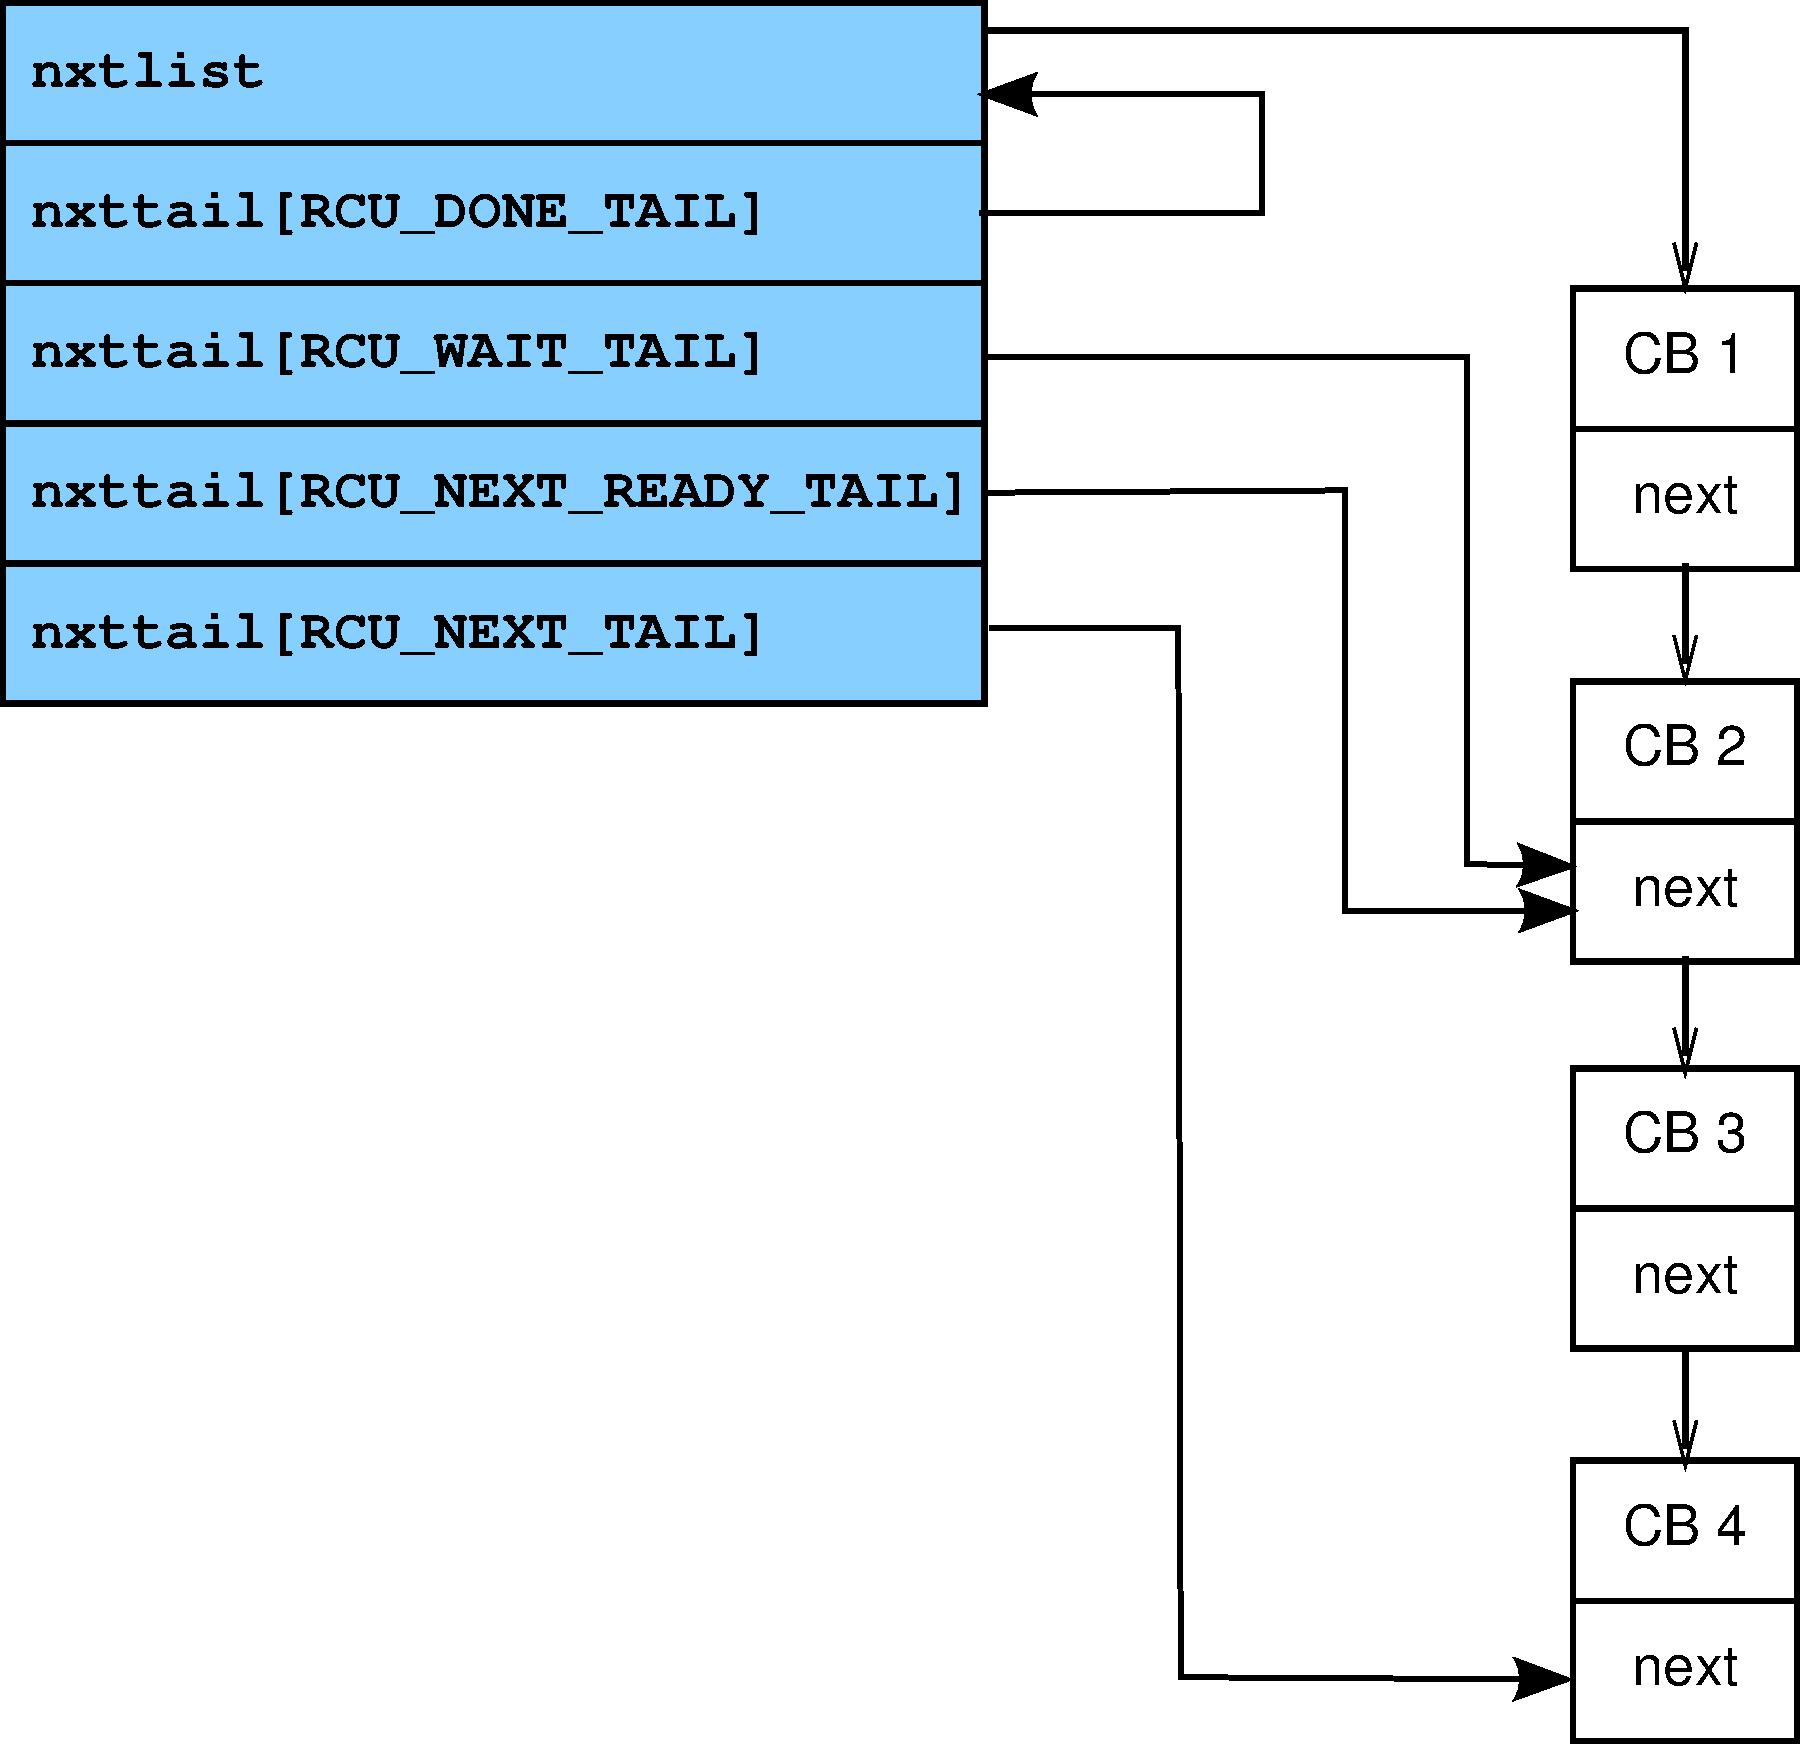
\includegraphics[scale=0.25]{rcu_data_callbacks.pdf}
\caption{Очередь callback'ов в \co{rcu_data}}
\label{fig:rcu_data_callbacks}
\end{figure}

%\comment{Lihao: since we don't model callbacks, only describe them briefly and add a reference
%to save space for the experiments section which is the main contribution of this paper.
%Do the same for discussion of preemptible RCU.}
\subsubsection{Callback'и RCU}
Структура \co{rcu_data} управляет RCU callback'ами, используя указатель
\co{->nxtlist}, указывающим на начало списка, и массив \co{->nxttail[]}
указателей-на-конец, формирующий четырехсегментный список
callback'ов~\cite{LaiJiangshan2008NewClassicAlgorithm},
где каждый элемент массива \co{->nxttail[]} указывает на конец
соответсвующего сегмента, как показано на рисунке~\ref{fig:rcu_data_callbacks}.
Сегмент, оканивающийся на \co{->nxttail[RCU_DONE_TAIL]}
(<<\co{RCU_DONE_TAIL} сегмент>>), содержит callback'и, связанные
с предыдущим grace-периодом, и, поэтому, готовые к вызову.
Сегменты \co{RCU_WAIT_TAIL} и \co{RCU_NEXT_READY_TAIL}
содержат callback'и, ожидающие окончания текущего и следующего
grace-периодов, соответственно.
Наконец, сегмент \co{RCU_NEXT_TAIL} содержит callback'и,
которые еще не были связаны с каким-либо grace-периодом.
%
Поле \co{->qlen} выполняет учет общего числа callback'ов,
а \co{->blimit} определяет максимальное число callback'ов,
которые могут быть вызваны в данный момент времени, тем самым
ограничивая размер окна времени, используемого для их вызова,
на длинных списках callback'ов.\footnote{
  Вычислительные окружения реального времени, требующие выполнения
  более строгих ограничений времени вызова, должны использовать
  callback offloading, который находится вне контекста данной статьи.}

Возвращаясь к рисунку~\ref{fig:rcu_data_callbacks} отметим,
что элемент массива \co{->nxttail[RCU_DONE_TAIL]} указывает на \co{->nxtlist},
что означает, что в данный момент ни один из callback'ов не готов к вызову.
Элемент \co{->nxttail[RCU_WAIT_TAIL]} указывает на \co{->next}-указатель
второго callback'а, что означает, что callback'и CB~1 и CB~2 ожидают окончания данного
grace-периода.
Элемент \co{->nxttail[RCU_NEXT_READY_TAIL]} указывает на тот же
\co{->next}-указатель, что означает, что список не содержит callback'ов,
связанных со следующим grace-периодом.
Наконец, callback'и, расположенные между \co{->nxttail[RCU_NEXT_READY_TAIL]} и
\co{->nxttail[RCU_NEXT_TAIL]} элементами (CB~3 и CB~4),
еще не связаны ни с каким grace-периодом.
Элемент \co{->nxttail[RCU_NEXT_TAIL]} всегда указывает либо на последний
callback, либо, если весь список пустой, на \co{->nxtlist}.

Cache locality достигается за счет вызова callback'ов на тех вычислительных ядрах,
которые их зарегистрировали.
Например, примитив записи RCU \co{synchronize_rcu()} добавляет
callback \co{wakeme_after_rcu()} в конец списка \co{->nxttail[RCU_NEXT_TAIL]}
на данном вычислительном ядре (Раздел \ref{sec:update_api_impl}).
По окончании данного grace-периода, которому соответствует изменение значения
поля \co{->completed} структуры \co{rcu_data}, меньшего, чем соответствующее значение
структуры \co{rcu_node}, они смещаются на один сегмент списка
(с помощью \co{rcu_advance_cbs()}).
Кроме этого, ядро процессора периодически объединяет сегменты \co{RCU_NEXT_TAIL}
и \co{RCU_NEXT_READY_TAIL} путем вызова \co{rcu_accelerate_cbs()}.
В некоторых специальных случаях, ядро выполняет объединение сегментов
\co{RCU_NEXT_TAIL} и \co{RCU_WAIT_TAIL}, пропуская сегмент \co{RCU_NEXT_TAIL}.
In a few special cases, the CPU merges the \co{RCU_NEXT_TAIL} segment
into the \co{RCU_WAIT_TAIL} segment, bypassing the \co{RCU_NEXT_TAIL}
segment.
Эта оптимизация применяется в тех случаях, когда ядро начинает новый grace-период.
Она \emph{не} используется, когда ядро обнаруживает новый grace-период,
поскольку этот период мог начаться до момента добавления callback'ов
в сегмент \co{RCU_NEXT_TAIL}.
%\comment{Lihao: why can't we invoke *all* callbacks when starting a new
%grace period? Isn't it true that all pre-existing read-side critical
%sections, i.e.~those start before callbacks are registered in \co{->nxttail}
%(in particular \co{wakeme_after_rcu} in \co{->nxttail[RCU_NEXT_TAIL]}),
%have finished?}
%\comment{Paul: In theory, we could, but in practice doing this would
%have several disadvantages:
%(1) All callbacks would be invoked by the grace-period kthread, and
%large systems could generate more callbacks than a single CPU could
%keep up with, which would delay subsequent grace periods and possibly
%even run the system out of memory.
%(2) Running all the callbacks at once could degrade real-time response.
%(3) Running callbacks on a different CPU than the one that registered
%them would decrease locality, increasing cache-miss rates, thus degrading
%performance.
%(4) This would require that atomic instructions be used when registering
%callbacks (as they are for no-CBs CPUs), further degrading performance.
%In addition, we could only invoke callbacks in the \co{RCU_NEXT_TAIL}
%segment, because callbacks in the later segments
%(\co{RCU_NEXT_READY_TAIL}, \co{RCU_WAIT_TAIL}, and
%\co{RCU_DONE_TAIL} might well have been queued \emph{after} the
%recently-completed grace period started.}
%
Это особенность архитектуры неслучайна: требование обеспечения
независимости работы вычислительных ядер
(для избегания исопльзования блокировок) является более важным,
чем сокращение продолжительности grace-периодов.
В тех редких случаях, когда требуются grace-периоды должны быть
максимально короткими, требуется использовать \co{synchronize_rcu_expedited()}.
Эта функция имеет такую же семантику, как и \co{synchronize_rcu()},
но предпочитает уменьшение задержки остальным оптимизациям.
% Lihao: this is where the callback of RCU's update API register?
% Paul: Yes, call_rcu() appends the callback to the end of the current
% CPU's RCU_NEXT_TAIL list.  Ignoring callback offloading for the moment.
% Lihao: we don't model QS forcing and offline CPUs
% Paul: Nor are you modeling callback offloading.  Which is fine, just calling
% it out.  ;-)

Каждый RCU callback представляет собой структуру \co{rcu_head},
имеющую поле \co{->next}, указывающее на следующий callback в списке,
и поле \co{->func}, указывающее на функцию, подлежащую вызову
по окончаниии предстоящего grace-периода.
